\documentclass[10pt]{article}

\usepackage[margin=1in]{geometry}
\usepackage{amsmath,amsthm,amssymb}
\usepackage{graphicx}
\usepackage{subfig}
\usepackage{float}
\usepackage{wrapfig}
\usepackage{multicol}
 \usepackage{booktabs}
 \usepackage{hyperref}
 \hypersetup{
 	colorlinks=true,
 	linkcolor=blue,
 	filecolor=magenta,      
 	urlcolor=cyan,
 }

\graphicspath{ {/Users/clay/Documents/research/TGE-SP21/assignments/images/} }

\begin{document}

% --------------------------------------------------------------
%                         Start here
% --------------------------------------------------------------

\title{Assignment 1}%replace X with the appropriate number
\author{Geosc 597-003\\
Techniques of Geophysical Experimentation} %if necessary, replace with your course title

\maketitle

\textit{\textbf{Objective(s):}
Build on in-class blinking an LED (diode).}

\section*{Activity 1 - Blinky 2}

Much like the in-class activity, we will control the blinking of \textbf{\textit{2 external LEDs}} on a breadboard. \\ \\
\noindent\textbf{Materials}
\begin{multicols}{2}
	{\small \begin{itemize}
		\item Arduino UNO
		\item USB Cable
		\item Breadboard
		\item LEDs (2 of your favorite colors)
		\item 330 $ \Omega $ resistors (Orange-Orange-Brown)
		\item M/M Jumper wires
		\item Computer (Mac, Linux, Windows)
	\end{itemize}}  
\end{multicols}

\noindent\textbf{Procedure}

\begin{itemize}
	\item Hook up the LEDs, resistors, and Arduino using the jumper wires and breadboard, similar to the in-class activity.
	
	\item LEDs are \textit{polarized} components meaning they have a certain way they need to be in the circuit. On LEDs the short leg next to the flat edge is the ground (-) connection.
	
	\item You will need to bend the legs of resistors to use them on the breadboard, you can do this with your hands or small pliers.
	
	\item Based on the code we used in the in-class Blinky activity, write a new program that blinks the LEDs in an alternating pattern.
	
	\item Get creative. What patterns can you make? Can you add more LEDs or change the pin assignment for each LED?
\end{itemize}

\begin{table}[h!]
	\footnotesize
	\centering
	\begin{tabular}{@{}ll@{}}
		\multicolumn{2}{c}{\textbf{Grading Rubric}} \\ \midrule 
		\multicolumn{1}{l}{\textit{Objective}}   & \textit{Points}   \\ \midrule 
		Code compiles                    & 10       \\ \midrule
		LEDs blink in patterns            & 15       \\ \midrule
		Total                            & 25       \\ \bottomrule
	\end{tabular}
\end{table}

% \clearpage
\section*{Activity 2 -  Stoplight}

In this activity you will make a simple single stoplight controller with an
Arduino UNO and some LEDs. You will become familiar with using the Arduino
programming environment and learn how to use the General Purpose Input/Output
(GPIO) pins on the microcontroller. You will also practice using good software
design technique by implementing well known design patterns and making
maintainable code. \\ 

\noindent\textbf{Materials}
\begin{multicols}{2}
	{\small \begin{itemize}
			\item Arduino UNO
			\item USB Cable
			\item Breadboard
			\item LEDs (Red, Yellow, Green)
			\item 330 $ \Omega $ resistors (Orange-Orange-Brown)
			\item 10k $ \Omega $ resistors (Brown-Black-Orange)
			\item Push button (momentary-on type)
			\item M/M Jumper wires
			\item Computer (Mac, Linux, Windows)
	\end{itemize}}  
\end{multicols}


\noindent\textbf{Procedure}

\begin{itemize}
	\item Connect the button, stop, caution, go, and left turn LEDs as shown in diagram.
	\item Start the Arduino IDE. Open the Blink example from: \textbf{File} $ \rightarrow $
	\textbf{Examples} $ \rightarrow $ \textbf{01.Basics} $ \rightarrow $ \textbf{Blink}. Read the comments and
	make sure you understand how it works.
	\item Connect your Arduino and hit the upload button.
	If it fails, check the board and port settings (in the *Tools* menu). Make
	sure the on-board LED is blinking to show a successful program upload.
	\item Change the pin number in the blink example to that of one of your LEDs. Make
	sure that the LED on the breadboard blinks, if not, you need to check the
	connections. Do this for each of the 4 LEDs.
	\item Draw a state machine diagram to meet the specifications of the attached
	requirements. Turn this in with the assignment!
	\item Build the state machine in the Arduino IDE and test it on your stoplight.
	Your final code should be commented, compile and run, and meet the
	specifications. Be sure to use good coding practices! Your code will be
	tested/graded by an identical Arduino setup.
\end{itemize}

\noindent\textbf{Requirements}
\begin{wraptable}{r}{5cm}
	%\begin{table}[h!t]
	\footnotesize
	\centering
	\begin{tabular}{@{}ll@{}}
		\multicolumn{2}{c}{\textbf{Grading Rubric}} \\ \midrule 
		\multicolumn{1}{l}{\textit{Objective}}   & \textit{Points}   \\ \midrule 
		Code compiles                    & 20       \\ \midrule
		Meets project requirements            & 30       \\ \midrule
		Total                            & 50       \\ \bottomrule
	\end{tabular}
	%\end{table}
\end{wraptable}
\begin{itemize}
	\item Begins in the red light state.
	\item Red light cycle lasts for 3 seconds.
	\item Yellow light cycle lasts for 1.5 seconds.
	\item Green light cycle lasts for 3 seconds.
	\item Works like a normal stoplight would, only one light on at a time and in the
	normal order (Red - Green - Yellow - Red).
	\item If a car was present in the left turn lane (simulated by holding down the push
	button) \textbf{before} the green light state, add a green left turn light for 2
	seconds. If no car is present, repeat the cycle.
	\item Uses the state machine implementation with functionalized code. No interrupts allowed!
\end{itemize}

\textbf{Example: } \url{https://www.youtube.com/embed/ltXPpmL2szE}

\clearpage

\begin{figure}[ht]
	\centering
	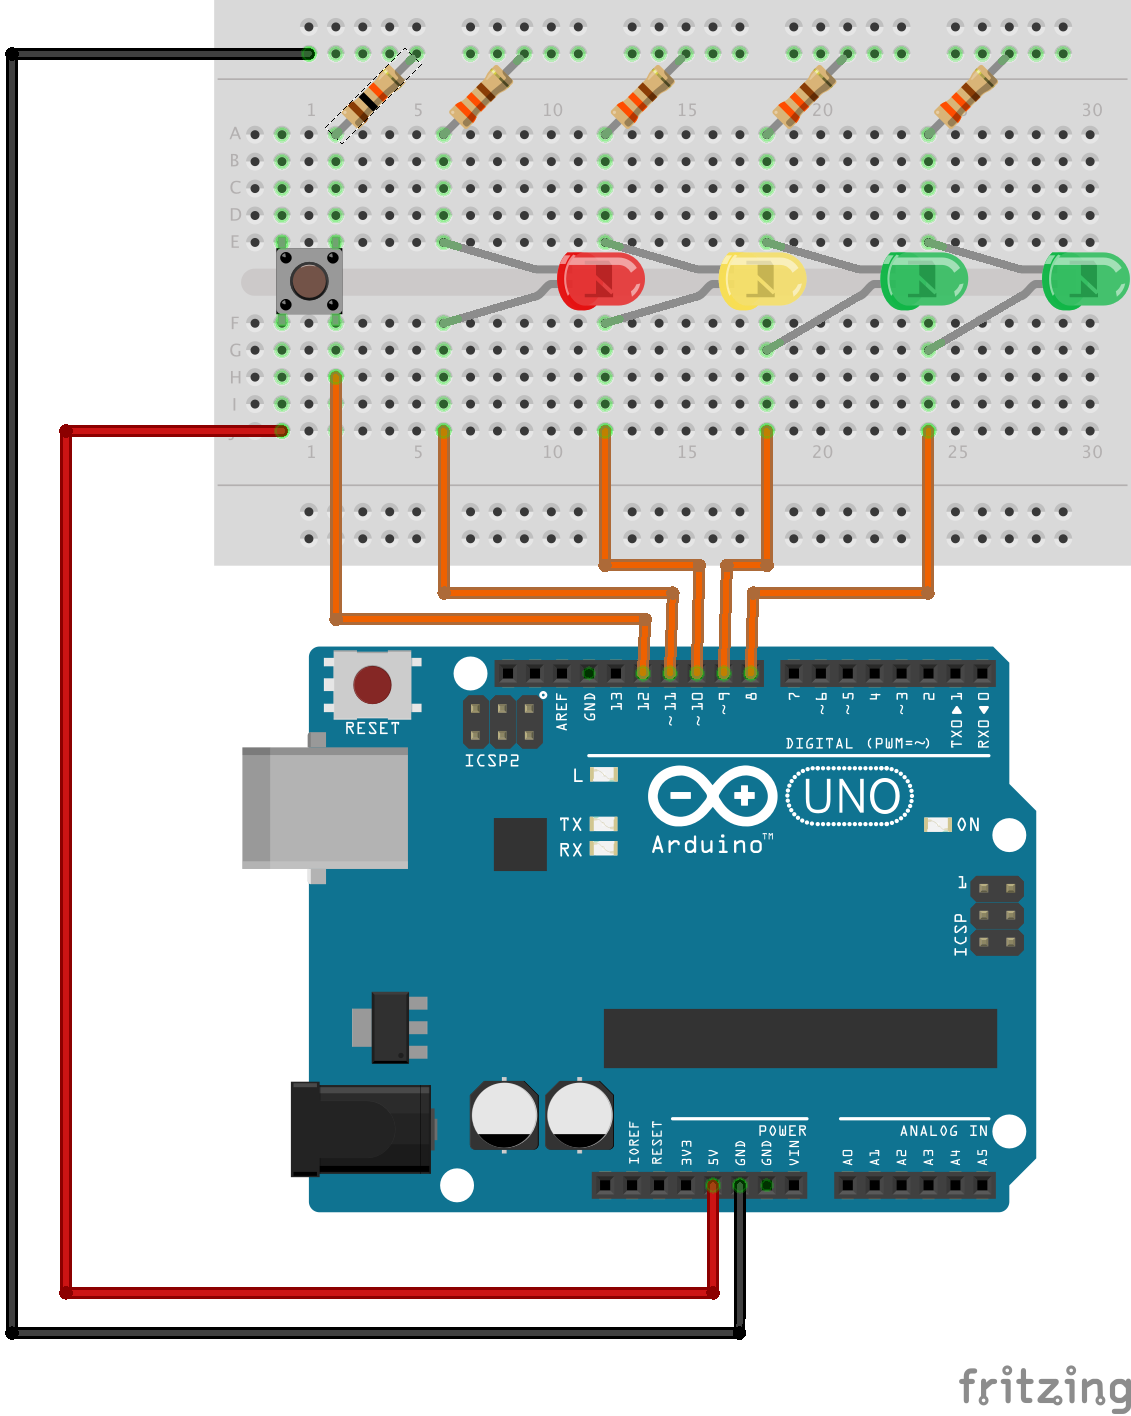
\includegraphics[width=0.5\columnwidth]{stoplight_fritzing}
	\caption{Wiring diagram for stoplight activity}
	\label{fig:stoplight_wiring_diagram}
\end{figure}



\end{document}